%======================================================================
\chapter{Related Work}
\label{chap:rw}
%======================================================================

\section{Object Segmentation}

Video object segmentation is the process of separating foreground objects from the background in a video~\cite{papazoglou2013}. A wide range of applications benefit from the progress of video object segmentation, e.g. robot-object interaction, recognition, video compression etc.

A variety of methods have been proposed to address the task~\cite{papazoglou2013,ma2012,wang2015,brox2010,taylor2015}. Most methods use motion cues to initialize the object segmentation.
A common method for motion detection is  background subtraction with mixture of Gaussians~\cite{kaewtrakulpong2002,zivkovic2004}. This technique models each pixel indepedently as a mixture of Gaussians but as it detects motion in each frame independently, the results lack completeness and temporal persistence.
In this paper, we address this shortcoming by modeling the appearance of objects from motion. 

Our proposed method treats moving pixels as a partial segmentation of objects and builds the appearance model for them, see Section~\ref{method-csc}. With the appearance model, those pixels that are not moving can successfully be classified as foreground or background to form a more complete segmentation. We model appearnce with Radial Basis Functions (RBF) as described in Section~\ref{method-csc}, an approach commonly used in interactive editing for selection propagation~\cite{li2010,tao2012}. We adapt the technique of Tao and Krishnaswamy~\cite{tao2012} but use motion detection instead of user selection to initialize the models.
 
Moving pixels obtained with background subtraction approaches may be not just incomplete, but also contain pixels from the background. This is mainly caused by shadows and noise. The consequence is that the computed segmentations are likely to cover regions that are not part of the foreground. We address this mis-classification with modeling background appearance and optimizing the classification. We use Graph Cuts~\cite{greig1989,boykov2004} to optimize the foreground and background classification based on the appearance model. To accelerate the computation, we divide frames into regions that contain one object each, see Section~\ref{method-tg}, and oversegment those regions with a fast superpixel method~\cite{siva2014} before classification, see Section~\ref{method-fbl}.

We evaluate our video object segmentation approach on a common dataset~\cite{f-li2013} in Section~\ref{dataset}. Our evaluation demonstrates that our approach achieves comparable results to two state-of-the-art approaches but our approach is on-line and is $10-200 \times$ faster than these methods.

The major contribution of our work is a fast on-line video object segmentation method that takes both motion and appearance of objects into account. We propose a novel integration of RBF appearance modeling and background subtraction through a Graph Cuts optimization on superpixels. We use local modeling to accelerate segmentation by dividing frames into regions that contain one foreground object each which greatly reduces the number of pixels to be processed. In Section~\ref{compression}, we propose an application of our on-line approach for compressing videos with compression quality adapted to foreground and background. The video object segmentation allows us to reduce the quality of the background by pre-processing it with a bilateral filter before compression while foreground objects are compressed as is by the compression scheme. We use H.264 coding.

A large number of methods have been proposed for extracting moving objects from an image sequence, using motion, depth, appearance or a combination of these cues.
Among those, motion is used most frequently as cues for object extraction~\cite{graciela2013} and many approaches use
background subtraction to this end~\cite{zeng2007,colombari2007}.
Classic background subtraction methods model the appearance of the background at each pixel and label the pixel that change rapidly to be foreground~\cite{jain1979,kaewtrakulpong2002,zivkovic2004}. These method typically assume a stationary or slowly panning camera.
More recently, optical flow is also used~\cite{ma2012,papazoglou2013,zhang2013,wang2015}.
The motion estimation algorithms typically provide pixel-wise labeling and errors are inevitable even using state-of-art algorithms.
To obtain robuster masks with semantic meaning, energy minimization is often used~\cite{papazoglou2013}.
Optical flow usually provides more motion cues than background subtraction (e.g. pixel correspondence accoss frames), but in general is much slower than background subtraction methods.
Our approach is closely related to tracking. We infer trimaps from detected motion to coarsely separate foreground from background, which is different from other methods based on motion cues~\cite{papazoglou2013,wang2015}.

With the advances in computational power of modern PCs and the progress of fast superpixel methods, the use of superpixels as units of object extraction are increasingly popular~\cite{papazoglou2013,wang2015,ochs2011}. Instead of naive superpixel voting schemes, researchers often use some optimization approaches to decide if a superpixel belongs to the foreground or the background~\cite{papazoglou2013,wang2015,ochs2011}. However, most of the superpixel methods are computationally intensive which prevents their use in real-time video object extraction~\cite{achanta2012}. A fast superpixel method was proposed by Siva and Wang~\cite{siva2014}. It is based on seam carving and dynamic programming and it achieves real-time performance in low resolution videos. We adapt this method and further accelerate the computation of superpixels by only segmenting the regions within the bounding boxes of foreground objects into superpixels.

Several video object extraction methods track points over the image sequences and then cluster the resulting point trajectories pairwise or in triplets~\cite{brox2010,ochs2011,ochs2012}.
The advantage of employing point tracking is the capacity of handling videos where moving objects are stationary in a number of frames.
The underlying assumption induced is that the objects are rigid so that all object points move according to a single translation~\cite{brox2010,ochs2011}, while the work of Ochs et al.~\cite{ochs2012} assumes a single similarity transformation. This assumption makes these methods not applicable to non-rigid objects.
The methods produce a sparse labeling in each frame, and superpixels are taken into account when turning the point trajectories into dense regions.
These methods are also able to handle partial occlusion but the drawback is that they are very slow (in the order of minutes per frame).

The work by Lee et al.~\cite{lee2011} shows the potential of using shape matching in object extraction.
The method first identifies object-like regions in any frame~\cite{endres2010}, followed by computing a series of binary partitions among those candidate regions to discover groups of shapes with persistent appearance and motion.
The drawbacks of this method include that it requires pre-processing identifying all object-like regions beforehand, it is very slow (in the order of minutes per frame), and it is not applicable to stationary or occluded (in some frames) foreground objects.

Depth information has been demonstrated to be robust to environment changes such as illumination change, dynamic backgrounds and camera motion~\cite{dahan2011,taylor2015}.
The work of Taylor et al.~\cite{taylor2015} infers depth layers from occlusion information. This gives it the capacity to be used outdoors and ensures it to be robust to occlusion and disocclusion. However, the method takes around 30 seconds for a VGA image on a standard desktop.

The works of Papazoglou and Ferrari~\cite{papazoglou2013} and Wang et al.~\cite{wang2015} are closely related to ours. Papazoglou and Ferrari~\cite{papazoglou2013} use optical flow as the motion cues. After generating a coarse segmentation, Graph Cuts are used to minimize an energy function containing an appearance term and smoothness terms. In this paper, we propose a novel algorithm based on Radial Basis Functions to model the appearance and estimate how close it is from a pixel to foreground or background, consindering the neighboring frames. We also use Graph Cuts to obtain the final masks.

Many modern approaches offer offline processing to recognize objects in videos~\cite{papazoglou2013,ma2012,wang2015,brox2010}. The requirement of the availability of the entire video limits those methods in processing long sequences.
In contrast, our method is online and offers processing in "streaming", which gives it the capacity to handle longer videos and integrate with other online applications.

\section{Remote Rendering}

Games, training, medicine and many other applications in everyday life~\cite{ramanathan2007,chun2011,kwon2017,rodriguez-gil2017} leverage the advantages of mobile devices with their rapidly progressing hardware and software.
The touch-based interaction on mobile devices is arguably more intuitive than the use of keyboard and mice on PCs. Nevertheless, mobile devices have their limitations when it comes to rendering and interacting with complex 3D models, e.g. lower processing power, limited storage and less capable rendering hardware.
Computationally intensive 3D graphics rendering tasks also impose severe challenges on the limited battery capacity of mobile devices.

To address these issues, remote rendering can be employed. This technique leverages the computational capacity of a remote server to relieve the rendering burden on the client side.
One direction in this field is partitioning and simplifying large and complex 3D meshes on a server and sending a part of simplified meshes to the client. Park and Lee~\cite{park2016} propose a framework to enable users to view large meshes on mobile devices hierarchically. Depending on various scales, meshes with different Level Of Detail (LOD) are generated on the server and transmitted to the clients.
However, transmission of meshes with different LOD frequently increases power consumption. Yan et al.~\cite{yan2014} propose the algorithm ASEHM that minimizes the transmission required in sending 3D meshes. Instead of transmitting a new level of the same model, ASEHM refines a coarser LOD into a higher-fidelity LOD, provided that the relationship between the LODs is available.

Another research direction is offloading the entire rendering task to the server. Basically, when a mobile client connects to the server, the server will initialize a rendering engine and an encoder for the mobile client. All the models are rendered on the server side and rendered frames are encoded and streamed from the server to the client as a video stream. Moreover, the server receives user interaction feedback from the client. This approach requires no 3D graphics capacity on the client and is able to use advanced encoding, such as H.264/AVC, to adjust the image quality according to the bandwidth availability.
Lamberti and Sanna~\cite{lamberti2007}, Moimark and Cohen-Or~\cite{noimark2003} and Lu et al.~\cite{lu2011} have proposed such CMR systems.
Many cloud gaming services and frameworks have leveraged this technology, e.g. OnLive~\cite{onlive}, NVIDIA GeForce Now~\cite{nvidia-geforce-now}, PlayStation Now~\cite{playstation-now} and Gaming Anywhere~\cite{gaming-anywhere}. Those services and frameworks use the cloud computing infrastructures to render the games and encode the rendered frames, while the clients decode the rendered frames and send the players' interactions to the cloud.
The primary disadvantage of this type of approach is the introduction of additional latency, including user interaction transmission time, rendering and encoding time at the server side, image transmission time, decoding time at the client side~\cite{shi2015}. However, minimizing the latency is challenging considering the high uncertainty of the network transmission. Using a geographically proximate server helps greatly reduce the latency since every 1000 miles of physical distance adds 25ms round-trip delay to the overall latency~\cite{perlman2010}.

To relieve the heavy dependence of remote rendering methods on the network, researchers proposed various methods~\cite{paravati2010,liang2009,yang2013}. One type of methods uses environment maps to accelerate rendering, e.g., 
Boukerche and Pazzi~\cite{boukerche2006} render environment maps on the server and send them to the client. With the environment map, the client is able to respond to the user interaction in the form of panning, tilting and zooming without latency. Evironment maps have some similarity to panoramas which were originally proposed by   
Chen~\cite{chen1995} in their QuickTime VR system which displayed virtual environments without rendering 3D models.
QuickTime VR accomplished moving through the environment by "hopping" to different panoramic points.
Boukerche and Pazzi~\cite{boukerche2006} do not simulate movement by "hopping" to another panoramic image, instead, they use a remote server to render panoramic images in real-time. They address the delay in rendering and transmitting panoramic images through a caching design that buffers visited viewpoints.
A common disadvantage of methods that use environment maps is that they only handle static environments and navigation typically leads to wait times for the user. If the objects in the scene move or the user navigates, re-rendering and re-transmission of environment maps can lead to latency~\cite{macchiavello2014,quax2016}.

Some researchers attempted to leverage the advantages of a depth map to synthesize new views on the client. 
Shi et al.~\cite{shi2012} proposed a framework that leverages depth maps to reduce user interaction latency. They take advantage of 3D image warping to synthesize the mobile display from the depth images generated on the server.
Chang and Ger~\cite{chang2002} proposed building Layered Depth Images (LDIs) on the server. The mobile device uses a 3D warping algorithm to synthesize the frame from a new view point.
At the time of the design of LDIs, mobile devices had almost no capacity to render 3D scenes and hence LDIs were designed as a way around to display 3D content on a mobile device. 
These image-based methods incorporating scene depth often face issues with visible gaps and holes in the rendered scene. Bao and Gourlay~\cite{bao2006-1,bao2006-2} proposed a method that uses a superview to direct the image warping and reduce the gaps and holes.
The method is successful in reducing the flaws in the synthetic images. But it is not designed to handle highly dynamic scenes, since a set of new reference depth maps need to be generated and delivered to the client whenever the scene changes. Their method is well suited for environment walkthrough applications but not for games and training applications.

Some other approaches support dynamic scenes and all types of interactions. They accelerate the data transmission in order to adapt to various network environments or reduce interaction delay.
Levoy~\cite{levoy1995} proposed a method that renders simplified models on clients to reduce bandwidth requirement. In this method, the server first renders both complete and simplified models and calculates a difference image between the two. Then the simplified model and the difference image are transmitted to the client. Finally, the client renders the simplified models and applies the difference image to produce a high-quality rendering. The simplification of models can be performed in terms of the textures and the number of polygons. This method reduces the bandwidth requirement for obtaining a high-quality rendering. Compared with our method, this work shares the same idea of using simplified models. But the difference is that Levoy~\cite{levoy1995} uses simplified models to achieve a compression effect on image transmission, while our method uses simplified models on the client side for display and interaction. Also, our simplification is selective and achieves a bandwidth reduction by rendering environment models only on the client.
Liu et al.~\cite{liu2014} extended image streaming and developed an automatic adaption algorithm that changes the rendering quality according to the network bandwidth. They use H.264 video encoding with fixed bit rate mode while adapting the rendering factors (e.g. view distance, realistic effect and texture detail) to improve the user experience. The goal of this method is to improve the visual quality of encoded frames with insufficient network bandwidth.
However, the rendering quality of all models is adapted at the same level since H.264 video encoding does not distinguish the importance of key models and environment models in a scene. Their work also does not address one of the most severe issues in remote rendering, interaction latency.
Hemmati et al.~\cite{hemmati2013bitrate} propose a method for cloud gaming, which selectively renders important objects and reduces video bitrate by not rendering unimportant objects. However, they did not answer the question about how it influences user experience.
Inspired by Hemmati et al.~\cite{hemmati2013bitrate}, Lu et al.~\cite{lu2017selective} proposed an approach that maximizes user experience with limited network bandwidth for stereo video streaming. In this approach, the left view and right view are rendered asymmetrically in terms of texture detail and certain objects are not rendered in on view. This technique enables intelligent decision of whether or not to render an individual object and how good the corresponding texture detail will be if rendered.

We propose a general-purpose remote rendering framework. On the one hand, by only rendering key models remotely, our method minimizes the network bandwidth requirement.
On the other hand, our method leverages the graphics capacity of mobile devices to loosen the tight dependence of the clients from the remote server. Applications using our framework are able to adapt to various network environments.
We do not assume a priori knowledge about the applications, thus our framework is able to handle dynamic scenes and all types of interaction (e.g. motion, panning and zooming). We also benefit from the increasing rendering capabilities of mobile devices while addressing the fact that mobile devices still fall behind PCs. We believe that the idea of offloading the entire rendering task to the server may be outdated given the recent advances in mobile device hardware.

\section{Augmented Reality Training}

The first augmented reality system can be dated back to 1962~\cite{johnson2010, yuen2011}. It employed a see-throught Head-Mounted Display (HMD). The HMD was tracked by a mechanical tracker and an ultrasonic tracker. However, only simple wireframes could be drawn and overlaid on the user's view due to the lack of computing capacity at that time~\cite{sutherland1968}. In 1992, Boeing~\cite{caudell1992} had already leveraged AR technology to assist their workers in assembling wire bundles.

The research and development for AR have gone on over the past five decades. The use of augmented reality technology has been explored in various fields, e.g. education, training, tourism, gaming, health, safty, etc~\cite{freitas2008,schrier2005,billinghurst2001}.
Freitas and Campos~\cite{freitas2008} developed an educational system using AR technology. The system teaches 2nd grade-level concepts, such as the means of transportation and types of animals. The system tracks a marker and superimposes the 3D models on the real-time video feed shown to the whole class. Experiments show that the nature of game-base learning of this system helps increase motivation among students~\cite{freitas2008}.
Schrier~\cite{schrier2005} developed a historic role-play game at a real site. The participants are assigned to a specific historic role and interact with virtual roles with a GPS-enabled mobile device.
Billings Hurst et al.~\cite{billinghurst2001} implemented a more interactive and realistic way of reading books. If the users look at the pages through a handheld AR display, they see 3D models appearing out of the pages.

There exist many reviews of implementations and progress in augmented reality applications~\cite{billinghurst2002,regenbrecht2005,zhou2008,lee2012}.
Billinghurst and Kato~\cite{billinghurst2002} focused on collaborative AR applications and demonstrated examples that allow people to view or change the same virtual models.
Regenbrecht et al.~\cite{regenbrecht2005} showed ten AR applications in various fields which make cutting edge progress at that time.
Zhou et al.~\cite{zhou2008} summarize the papers published on ISMAR from 1997 to 2007 in an statistical way. They focus on analyzing the frequency and percentage of citations of each topic involved in augmented reality applications.
Lee~\cite{lee2012} discussed the areas that augmented reality technology has been used in and identify how it can be used in each area.
We present a new methodology to categorize existing applications of augmented reality in the remaining part of this section.

In this section, we focus on the use of augmented reality technology in training. After reviewing recent progress in this area, we propose a new methodology of categorizing the AR applications. We categorize them into two categories in terms of interactive targets: real objects and virtual objects. Fig.~\ref{fig:category} shows two examples, where the left one shows that a trainee is interacting with a real object, and the right one depict that a trainee is interacting with a virtual object. When interacting with a real object, the overlaid virtual ones act as an instruction that guides the trainee through the process.

\begin{figure}
	\centering
	\subfigure[Interact with real objects]{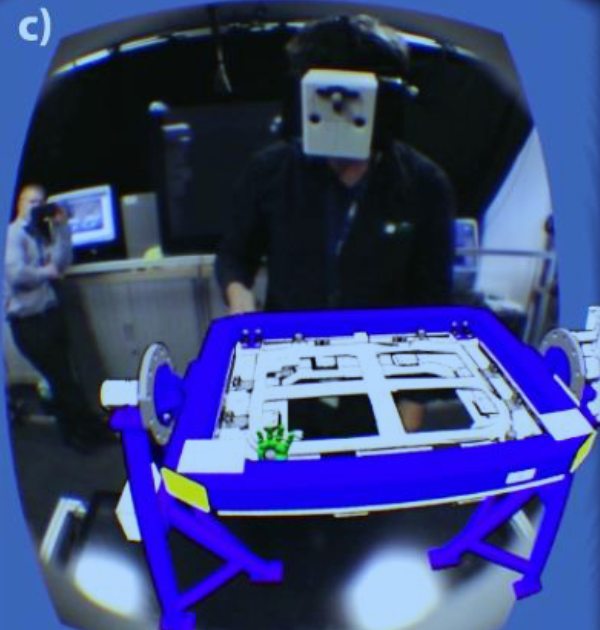
\includegraphics[width=0.35\columnwidth]{figures/category2.png}}
	\subfigure[Interact with virtual objects]{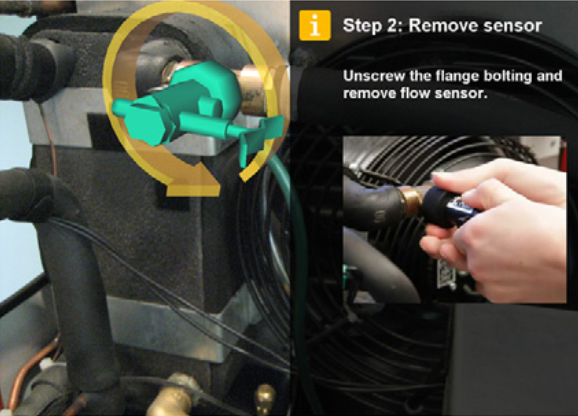
\includegraphics[width=0.51\columnwidth]{figures/category1.png}}
	\caption{Two categories of augmented reality training scenarios according to which objects people interact with.}
	\label{fig:category}
\end{figure}

\subsection{Virtual Objects} In the framework depicted in~\cite{nakajima2003}, the camera captures the images of a participant standing in front of a blue screen. The participant uses a "wand" to interact with a virtual environment, where the "wand" can be a finger, a fire extinguisher or other things we have seen in normal life. There is no marker needed to recognize the position and orientation of the "wand".
Luo et al.~\cite{luo2005} developed an AR-based therapy application that was designed for post-stroke finger extension rehabilitation. The application involves both therapists and the patients. During the rehabilitation, the patients need to wear a head-mounted display and an orthosis. The virtual objects prepared by the therapist are mixed with the patient's hand and displayed on the head-mounted display. When the patient is trying to grasp or release the virtual object, the on-site therapist adjusts the assistance provided by the orthosis.
Leblanc et al.~\cite{leblanc2010} compared an AR training method with the traditional methods in the field of straight laparoscopic colorectal skills acquisition training. The traditional methods cost much higher than the the AR training method since it uses human cadavers. They conclude that simulator training followed by cadaver training can appropriately integrate simulators into the learning curve and maintain the benefits of both training methodologies.
Nishino et al. present a Japanese calligraphy training system to teach learners how to write better characters~\cite{nishino2011}. It allows the learners to watch and feel the writing techniques of an instructor. More specifically, the training system displays a virtual brush and enables the learners to intuitively master instructor's motor skills through the sense of touch with a haptic device.
Gonzalez-Franco et al.~\cite{gonzalez-franco2016} developed an approach for training in complex manufacturing scenarios, where the virtual objects are projected into real scenes without their real counterparts. The trainers operate on the virtual objects with a wand to teach the trainees. In this use case, the interactive targets are the virtual objects.

The methods in this category are usually applied on the fields where the cost or risk of real hands-on experience is too high. For example, a surgeon could use AR to learn how to perform open-heart surgery without risking patients' lives.

\subsection{Real Objects} In engineering, especially in the field of machine maintenance and repairing, the cost of real hands-on experience is relatively low, but the complexity of the target is very high. In this kind of scenarios, people often use augmented reality technology to show virtual objects as a guide.

Boeing proposed the first industrial augmented reality application that helps its workers with assembling aircraft wire bundles~\cite{caudell1992}. Henderson and Feiner developed a framework to assist conducting military routine maintenance tasks inside an armored vehicle turret~\cite{henderson2009}. The experiment shows that use of AR increases the precision of component locating by 56\% compared with the use of traditional untracked head-up displays (HUDs) and speeds up the task by 47\% compared with standard computer monitors.
Crescenzio et al.~\cite{crescenzio2011} implemented an AR-based maintenance tool for daily inspections of the Cessna C.172P, an airplane often used by flight schools. It superimposes digital replicas of parts and subparts or graphical symbols to attract the operator's attention and guide the technicians through a task. It uses a markerless, feature-based method for HMD registration. What is more interesting is that they also provide an authoring tool for new training material generation. By leveraging the CAD models and existing scanning tools, a trainer can generate new training materials without the knowledge of programming. However, it still requires a lot of efforts to scan real scenes for locating the virtual objects in the real scenes.

Hincapi� et al.~\cite{hincapie2011} demonstrated an AR-based training process to perform maintenance on the body of the RV-10 aircraft. The system overlays virtual objects onto real objects as an instruction. Trainees need to work on the RV-10 aircraft component based on the instructions.
Webel et al.~\cite{webel2011,webel2013} proposed a framework for assembly and maintenance training. The trainees operate on a real machine, while the instructions are shown by overlaying a virtual machine on the real one. In this work, the interactive targets are the real objects, while the virtual ones are shown as the instruction.

Most of existing methods generally guide the user through a fixed series of steps and the digital content is prepared beforehand. The topic of augmented reality training material authoring is overlooked in this research area. Zhou et al.~\cite{zhou2008} conclude that only 3.8\% papers published on ISMAR from 1997 to 2007 discussed about authoring but made 8.9\% of citations.
However, we cannot find existing work on real-time authoring tools.
Wang et al.~\cite{wang2010} developed an authoring tool for AR-based examinations. Providing 3D models involved in exam questions, the application generates the AR content and stores it in a separate file that can be shared, edited or imported into an AR interface.
Anderson et al.~\cite{anderson2013} proposed a movement training application that is equipped with a human motion recording tool. They record people's movements and present them in an augmented reality mirror, and the users can see their mirror image as well as the targeting movements in the mirror and follow those movements.
However, they are still not real-time authoring tools, since the content need to be prepared or captured before the training.
Moreover, during the training, the applications collect minimal feedback from the user and cannot adjust according to the user's performance or mistakes.
Missing real-time authoring tools and the lack of just-in-time feedbacks place an obstacle between the trainer and the trainee.
Our proposed framework bridges the gap between the trainer and the trainee.
On the one hand, guides or instructions are not fixed but generated by the trainer in real time instead. On the other hand, the steps taken by trainees are collected and sent to trainers, so that trainers are able to evaluate the trainees' performance and correct mistakes.
